% Document class.
\documentclass{article}
% Colors etc
\usepackage{color}
\usepackage[usenames,dvipsnames]{xcolor}
\definecolor{light-gray}{gray}{0.95}
% Hyphonation for text and url
\usepackage[english]{babel}
\usepackage[hyphens]{url}

\usepackage{pdfpages}

%Enable bibliography
\usepackage[numbers,sort&compress]{natbib}
\bibliographystyle{plainnat}

% Accept é ë etc
\usepackage[utf8]{inputenc}
\usepackage[T1]{fontenc}
% Thanks, Laura Baakman

% \usepackage{eso-pic}

% More fonts and symbols
\usepackage{textcomp}
\usepackage{amsfonts}

% Allow for more symbols etc
\usepackage{verbatim}
\usepackage{marvosym}
\usepackage{amsmath}

% Math... and stuff
\usepackage{mathtools}

% Listings and other mark up
\usepackage{listings}
\usepackage{appendix}


% Define the style of lstlisting
\lstset{ %
language=matlab,        						% choose the language of the code
basicstyle=\ttfamily,       				% the size of the fonts that are used for the code
numbers=left,        	          			% where to put the line-numbers
numberstyle=\footnotesize,			      	% the size of the fonts that are used for the line-numbers
stepnumber=5,                   			% the step between two line-numbers. If it's 1 each line will be numbered
firstnumber=1,								% changes the first number
numberfirstline=true						% numbers the first line and ensures the rest are multiples of 5.
numbersep=5pt,                  			% how far the line-numbers are from the code
backgroundcolor=\color{light-gray},  		% choose the background color. You must add \usepackage{color}
showspaces=false,               			% show spaces adding particular underscores
showstringspaces=false,         			% underline spaces within strings
showtabs=false,                 			% show tabs within strings adding particular underscores
tabsize=2,                    				% sets default tabsize to 2 spaces
captionpos=b,                   			% sets the caption-position to top
breaklines=true,                			% sets automatic line breaking
breakatwhitespace=false,		        	% sets if automatic breaks should only happen at whitespace
escapeinside={\%*}{*)}          			% if you want to add a comment within your code
}
% Thanks to Dirk Zittersteyn

% Graphics like pictures
\usepackage{graphicx}
\usepackage{graphics}
\usepackage{caption}
\usepackage{subcaption}
\usepackage{wrapfig}
\usepackage{epsfig}
\usepackage{titlesec}
\usepackage{float}
\usepackage{siunitx}
\usepackage{parskip}
\usepackage{hyperref}

\begin{document}


\begin{titlepage} % Suppresses displaying the page number on the title page and the subsequent page counts as page 1
	\newcommand{\HRule}{\rule{\linewidth}{0.5mm}} % Defines a new command for horizontal lines, change thickness here
	
	\center % Centre everything on the page
	
	%------------------------------------------------
	%	Headings
	%------------------------------------------------
	
	\textsc{\LARGE WEB AND CLOUD COMPUTING 2017}\\[1.5cm] % Main heading such as the name of your university/college
	
	%\textsc{\Large Major Heading}\\[0.5cm] % Major heading such as course name
	
	%\textsc{\large Minor Heading}\\[0.5cm] % Minor heading such as course title
	
	%------------------------------------------------
	%	Title
	%------------------------------------------------
	
	\HRule\\[0.4cm]
	
	{\huge\bfseries Project: Uber for Bikes}\\[0.4cm] % Title of your document
	
	\HRule\\[1.5cm]
	
	%------------------------------------------------
	%	Author(s)
	%------------------------------------------------
	\textsc{\large Group 18}\\[0.5cm] % Minor heading such as course title
	
	\begin{minipage}{0.6\textwidth}
		\begin{center}
			\large
			\textit{Authors}\\
			\textsc{Thom Carretero Seinhorst} \\ % Your name
			\textsc{Alexandru Tatarov} \\% Your name
			\textsc{Anastasia Serebryannikova} % Your name
		\end{center}
	\end{minipage}
	~
	
	
	% If you don't want a supervisor, uncomment the two lines below and comment the code above
	%{\large\textit{Author}}\\
	%John \textsc{Smith} % Your name
	
	%------------------------------------------------
	%	Date
	%------------------------------------------------
	
	\vfill\vfill\vfill % Position the date 3/4 down the remaining page
	
	{\large\today} % Date, change the \today to a set date if you want to be precise
	
	%------------------------------------------------
	%	Logo
	%------------------------------------------------
	
	%\vfill\vfill
	%\includegraphics[width=0.2\textwidth]{placeholder.jpg}\\[1cm] % Include a department/university logo - this will require the graphicx package
	 
	%----------------------------------------------------------------------------------------
	
	\vfill % Push the date up 1/4 of the remaining page
	
\end{titlepage}


\section{Introduction}

In this project we developed a single page web application "Uber for bikes". The final goal was to create something similar to the Uber functionality for bikes.

The application represents a map on which the positions of the bikes are shown. These bikes are used by people
for transportation. Users can also see the table with the address information about the bikes. The coordinates of the bikes are streamed from the database and then transformed into addresses using Google Maps API. The user can book a bike by pressing the corresponding button. When a bike is taken, its corresponding point on the map disappears (because it is no longer available) for all users except the user who reserved it. For that user the marker's position will be updated every 10 seconds in order to help the user reach the destination point easier. When the trip is finished the bike appears back on the map. 



\section{Architecture}
In \autoref{arch}, a broad overview of the architecture of the application is given. 

    \begin{figure}[H]
		\centering
		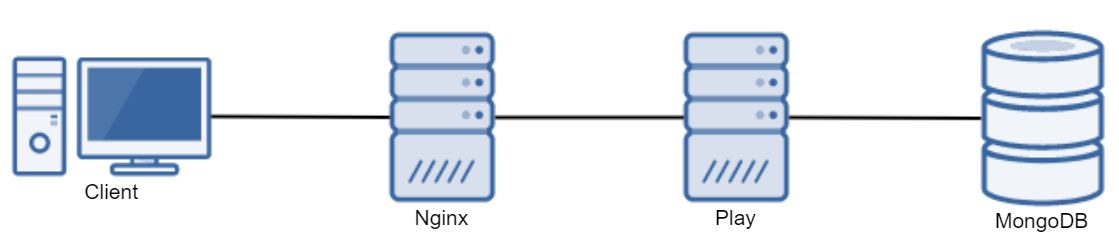
\includegraphics[width=1.0\textwidth]{images/Architecture.png}
		\caption{Overview of the architecture of Uber for Bikes}
		\label{arch}
	\end{figure}
	
An instance of the application has several virtual machines running so that each could be placed on different hardware. 

For our webserver we have written the main component in Scala. Scala is functional programming language supporting high scalability. To write not everything from scratch, we used the Play Framework. 

For our project we used for our database MongoDB with ReactiveMongo. ReactiveMongo is a Scala driver that provides fully non-blocking and asynchronous I/O operations. ReactiveMongo is designed to avoid any kind of blocking request. Every operation return immediately, freeing the running thread and resuming execution when it is over.

In the frond-end AngularJS and Bootstrap is used for providing a nice user interface. The UI serves a simple purpose: Renting and unrenting bikes. The main view of the UI is a Google Maps view. It is currently set to the location of Groningen, but could eventually be used to show the region where the user resides.
In our project we use an external third party service. The service of Google is needed to convert a textural representation of a location into the corresponding geographical representation of the GPS system. This conversion is done via the Google Maps API.


\subsection{Docker swarm}

Explain the docker swarm


%\section{Technologies}




\section{Design decisions}

\subsection{Database}
We use MongoDB for our database. We chose to use this database as it is easy to implement and easy to use. We have
a MongoDB database with 1 collection, Bikes. The Bikes collection stores all bike locations and their availability. There should be a second database collection, Users, for storing the name, passwords and a list of rented bikes. Due to lack of time, we weren't able to implement this correctly.


    \begin{figure}[H]
		\centering
		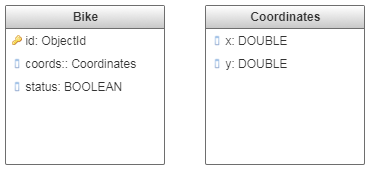
\includegraphics[width=0.4\textwidth]{images/db-structure.png}
		\caption{Overview of the database}
		\label{database}
	\end{figure}


\subsection{Webserver}
We chose Play as the framework for back-end development of our application mostly because it supports asynchronous I/O. There were two main causes for choosing Scala: the first is the possibility to learn a new programming language and the second is professor's incentive to use Scala for back-end development. In the end we succeeded in building a working back-end. We benefited from online completed projects we found on the internet as it aided our understanding and development of the final product. During the development we had difficulties connecting our database with Play as well as using WebSockets for live data streaming.

\subsection{Client}
Angular is a framework for building Web single-page applications and Bootstrap is an easy to use front-end web framework for designing web applications. These are the main reasons why we chose to use these frameworks. Other advantage of using Angular is its highly readable and comprehensive code. It was an important factor because we wanted something that will take as little time to learn as possible. We created the project using Angular Cli and used components to create the navigation bar, map component, and two (login and registration) forms (unfortunately not seen in the final layout). Even if it is not linked to framework itself, we found useful the large community of developers using Angular as online answers helped us solve most encountered problems.

\begin{figure}[H]
		\centering
		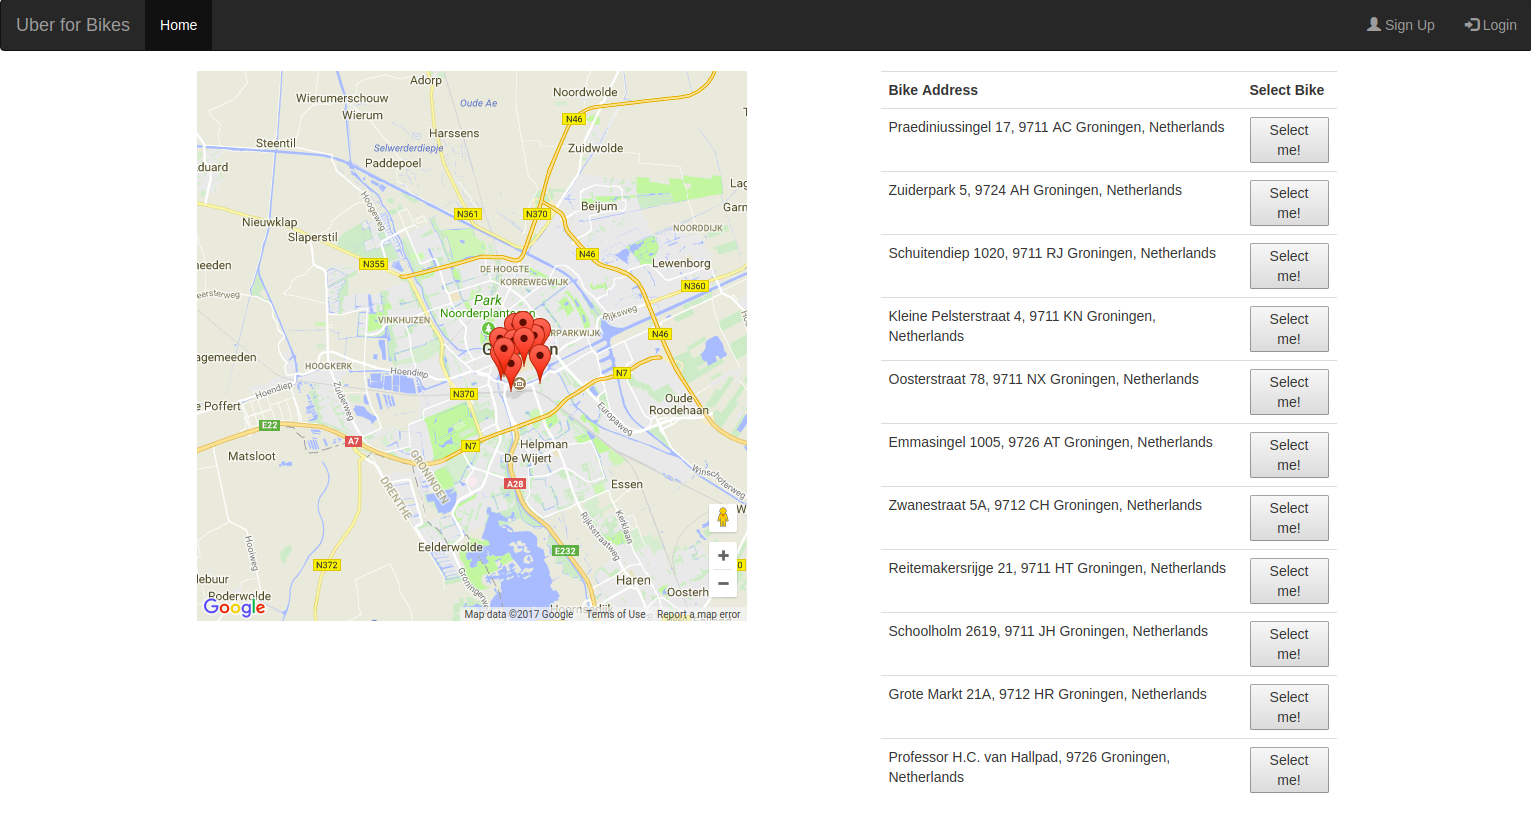
\includegraphics[width=0.9\textwidth]{images/screenshot.png}
		\caption{Application layout}
		\label{front-end}
	\end{figure}



\section{Discussion}

In this chapter we review and reflect on the project.

At the beginning of the project we started with developing an UI. After that we created an nginx webserver and implemented a backend service using Play framework, but we struggled a lot to provide the connection from the front-end to the back-end. It took us quite a lot of time to figure it out how exactly to connect all the parts together. We ended up using Rest API  to connect the front-end to the back-end. We also tried to implement WebSockets. At the end we finally managed to successfully retrieve the data from the database and to present it in the UI. As already mentioned, we chose to use Angular as a framework for our UI.

It took us some time to set up the back-end with Play and Scala. Since the programming language Scala was new to all of us, we had to put some time and effort in understanding how Scala works.

\subsection{Angular}
Angular proved to be the easiest component of the project.  However not everything was straightforward. One tricky part was using Ajax calls to retrieve information about available bikes and displaying it. We needed a little more time than expected to use the values from \textit{.subscribe()} in some other function.
\subsection{Scala}
Scala was completely new to all of us. We were lucky enough to find a project that provided some similar functionalities. Using that project as a guideline, we implemented a part of our own back-end functionality that communicates with front-end and the database. The biggest issue we encountered at using Scala was implementing WebSockets because we could not find many examples online.
\subsection{Docker}
Docker appeared to be an extremely nice tool for developing applications. With Docker, it has become very easy to separate the infrastructure decisions from the internal application issues. Docker was pretty easy to learn and quite easy to use. The documentation appears to be more or less comprehensive and Docker itself seems to be very user-friendly. The main issues that we had in this part were mainly connected to deploying certain containers and figuring out the correct settings for them. For example, sbt failed to dockerize our Play application, so we had to discover an alternative way to do that. Replicating MongoDB instances and importing data in the database also caused some problems. However, the docker logic overall seemed to be very straightforward and did not cause significant issues.

Docker swarm mode that we used in our application appears to be extremely useful in providing fault tolerance and its logic is easy to understand. It enables fault tolerance in a very intuitive way by replicating the services among different nodes in the cluster or even within a single node. Getting acquainted with Docker definitely was one of the most valuable and beneficial tasks during this course.

\subsection{Future work}
Probably the most important feature that is missing is the live streaming of the data. It was supposed that the bike locations would change every 10 or 30 seconds in correspondence to the real ones. Another important part of the project that is missing is the login and register part for the users of the application. By saying that it is missing we mean that it is not functional. The form components have been created, but they do nothing when \textit{Submit} button is pressed. Users should be able to create an account and to login. When a user is logged in, he can rent a bike and see his history of rented bikes. This history can vary from just the day and the coordinates/address of the start and end points to a map that shows all the intermediary points recorded using live data streaming. Another missing part is the history of the bike. Due to the difficulties we encountered there was not enough time to implement this correctly. Finally, some stylistic upgrades can be done. However this is not important in the context of the functionality of the project, which now represents a fully connected functioning system.


%\bibliographystyle{plainnat}
%\bibliography{refs}
\end{document}